\documentclass[12pt]{article}
\setlength{\oddsidemargin}{0in}
\setlength{\evensidemargin}{0in}
\setlength{\textwidth}{6.5in}
\setlength{\parindent}{0in}
\setlength{\parskip}{\baselineskip}
\usepackage{amsmath,amsfonts,amssymb}
\usepackage{graphicx}
\usepackage{enumitem}
\usepackage[]{algorithmicx}
\usepackage{amsthm}
\usepackage{fancyhdr}
\pagestyle{fancy}
\setlength{\headsep}{36pt}
\usepackage{tkz-berge}
\usetikzlibrary{positioning, automata}

\usepackage{hyperref}

\theoremstyle{remark}
\newtheorem*{solution}{Solution}

\newcommand{\makenonemptybox}[2]{%
%\par\nobreak\vspace{\ht\strutbox}\noindent
\item[]
\fbox{% added -2\fboxrule to specified width to avoid overfull hboxes
% and removed the -2\fboxsep from height specification (image not updated)
% because in MWE 2cm is should be height of contents excluding sep and frame
\parbox[c][#1][t]{\dimexpr\linewidth-2\fboxsep-2\fboxrule}{
  \hrule width \hsize height 0pt
  #2
 }%
}%
\par\vspace{\ht\strutbox}
}
\makeatother

\begin{document}
\definecolor {processblue}{cmyk}{0.96,0,0,0}

\lhead{{\bf CSCI 3104, Algorithms \\ Problem Set 4b (45 points)} }
\rhead{Name: \fbox{Michael Rogers} \\ ID: \fbox{105667404} \\ {\bf Profs.\ Hoenigman \& Agrawal\\ Fall 2019, CU-Boulder}}
\renewcommand{\headrulewidth}{0.5pt}

\phantom{Test}

\begin{small}
\textbf{Instructions for submitting your solution}:
\vspace{-5mm} 

\begin{itemize}
	\item The solutions \textbf{should be typed} and we cannot accept hand-written solutions. \href{http://ece.uprm.edu/~caceros/latex/introduction.pdf}{Here's a short intro to Latex.}
	\item You should submit your work through \href{https://www.gradescope.com/courses/59294}{\textbf{Gradescope}} only.
	\item If you don't have an account on it, sign up for one using your CU email. You should have gotten an email to sign up. If your name based CU email doesn't work, try the identikey@colorado.edu version. 
	\item Gradescope will only accept \textbf{.pdf} files (except for code files that should be submitted separately on Gradescope if a problem set has them) and \textbf{try to fit your work in the box provided}. 
	\item You cannot submit a pdf which has less pages than what we provided you as Gradescope won't allow it. 
	\item Verbal reasoning is typically insufficient for full credit. Instead, write a logical argument, in the style of a mathematical proof.
	\item For every problem in this class, you must justify your answer:\ show how you arrived at it and why it is correct. If there are assumptions you need to make along the way, state those clearly.
	
	\item You may work with other students. However, \textbf{all solutions must be written independently and in your own words.} Referencing solutions of any sort is strictly prohibited. You must explicitly cite any sources, as well as any collaborators. 
\end{itemize}



\vspace{-4mm} 
\end{small}

\hrulefill

\newpage
\begin{enumerate}

\item (10 pts) For a directed graph with positive weights, we define the max-weight of a path from $s$ to $d$ as the maximum of the edge weights along the path. For example, if the path from A to D has edges and weights of $e_{AB} = 5$, $e_{BC} = 4$, and $e_{CD}=1$, the length of the path is defined as $e_{AB} + e_{BC} + e_{CD}$, and the max-weight is 5.
\begin{enumerate}
\item(5 pts) Give an algorithm to compute the smallest max-weight paths from a source vertex s to all other vertices. In this problem, you are changing the definition of length of the path from A to D to $max(e_{AB}, e_{BC}, e_{CD})$ (Hint: Your algorithm should be a modification of Dijkstra's algorithm presented in Lecture.)\\ \\

\begin{verbatim}
def shortestPath(G,s): 
   dist(s) = 0 
   dist(v) = Infinity for all v-s
   max = 0
   Q = Min priority queue
   Q.add(All v in G)
   while Q ! empty:
      u = Q.pop()
      for each v in u.adj:
         d = dist(u) + e(u,v)
         if d > dist(u):
            dist(u) = d
            prev(v) = u
            if d > max:
               max = e(u,v)
   return G
\end{verbatim}

\pagebreak
\item(5 pts) Prove the correctness of your algorithm.
\end{enumerate}
\begin{solution}

\end{solution}

\pagebreak

\item (11 pts) Based on the following graph :
\begin{figure}[h!]
\begin{center}
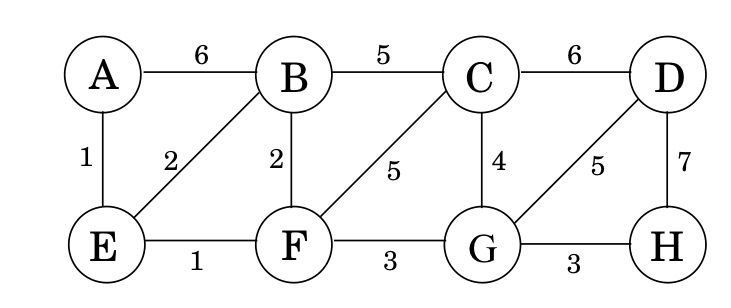
\includegraphics[scale=0.3]{mst_graph_q2.jpg} 
\end{center}
\end{figure}

\begin{enumerate}[label=(\alph*)]

\item (4 pts) In what order would Prim's algorithm add edges to the MST if we start at vertex $A$? 
\begin{solution}
(A,E),(E,F),(E,B),(F,G),(G,H),(G,C),(G,D)
\end{solution}
\pagebreak
\item (7 pts) In what order Kruskal's would add the edges to the MST? For each edge added by Kruskal's sequentially, give a cut that justifies it's addition. 
\begin{solution}

\end{solution}
 

\end{enumerate}

\pagebreak

\item (10 pts) Let $T$ be a MST of a given graph $G$. Will $T$ still be the MST if we reduce the weight of exactly one of the edges in $T$ by a constant \textbf{c}? Prove your answer.
\begin{solution}

\end{solution}

\pagebreak
\item (14 pts) One of the uses of MSTs is finding a set of edges that span a network for minimum cost. Network problems could also have another type of objective: designing a spanning tree for which the most expensive edge is minimized. Specifically, let $G = (V, E)$ be a connected graph with $n$ vertices, $m$ edges, and positive edge costs that you may assume are all distinct. Let $T = (V, E)$ be a spanning tree of $G$; we define the \textbf{limiting edge} of $T$ to be the edge of $T$ with the greatest cost.
A spanning tree $T$ of $G$ is a minimum-limiting spanning tree if there is no spanning tree $T$ of $G$ with a cheaper limiting edge.
\begin{enumerate}
\item (7 pts) Is every minimum-limiting tree of $G$ an MST of $G$? Prove or give a counterexample.
\begin{solution}

\end{solution}

\pagebreak
\item (7 pts) Prove that every MST of $G$ is a minimum-limiting tree of $G$. [\textbf{Hint:} Let $T$ be an MST of $G$, and let $T^{\prime}$ be a minimum-limiting tree of $G$. If $T$ is not a minimum-limiting tree, can we replace the heaviest edge of $T$? Think about how to use $T^{\prime}$ here.]

%Is every MST of $G$ a minimum-limiting tree of $G$? Prove or give a counterexample.
\begin{solution}

\end{solution}

\end{enumerate}

\end{enumerate}

\pagebreak
\textbf{Ungraded questions} - These questions are for your practice. We won't grade them or provide a typed solution but we are open to discuss these in our OHs and you should take feed backs on your approach during the OHs. These questions are part of the syllabus. 

\begin{enumerate}

\item Suppose you are given the minimum spanning tree $T$ of a given graph G (with $n$ vertices and $m$ edges) and a new edge $e=(u,v)$ of weight $w$ that will be added to $G$. Give an efficient algorithm to find the MST of the graph $G\cup e$, and prove its correctness. Your algorithm should run in $O(n)$ time.\\
\begin{solution}

\end{solution}

\item Based on the following graph :
\begin{figure}[h!]
\begin{center}
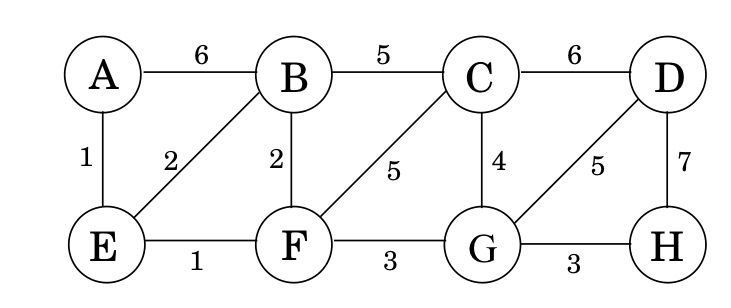
\includegraphics[scale=0.3]{mst_graph_q2.jpg} 
\end{center}
\end{figure}

\begin{enumerate}[label=(\alph*)]

\item Run Kruskal's and find the MST. You can break the ties however you want. Draw the MST that you found and also find it's total weight.
\begin{solution}

\end{solution}
\pagebreak
\item Run Prim's starting from vertex $A$ and find the MST. You can break the ties however you want. Draw the MST that you found and also find it's total weight. Is the total weight same as what you get from the above?
\begin{solution}

\end{solution}
 
\end{enumerate}

\item Consider the following unweighted graph, and assign the edge weights (using positive integer weights only), such that the following conditions are true regarding minimum spanning trees (MST) and single-source shortest path (SSSP) trees:
	\begin{itemize}
	\itemsep-0.1pt
	\item The MST is distinct from any of the seven SSSP trees.
	\item The order in which Prim's algorithm adds the safe edges is different from the order in which Kruskal's algorithm adds them.
	\end{itemize}
	Justify your solution by (i) giving the edges weights, (ii) showing the corresponding MST and all the SSSP trees, and (iii) giving the order in which edges are added by each of the three algorithms. 	
	\begin{figure}[h!]
\begin{center}
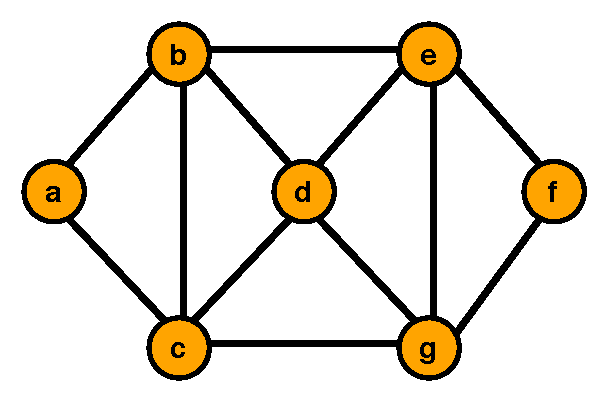
\includegraphics[scale=0.6]{graph_mst.pdf} 
\end{center}
\end{figure}

\begin{solution}

\end{solution}

\end{enumerate}

\end{document}
